\documentclass{article}
\usepackage[utf8]{inputenc}
\usepackage[spanish]{babel}
\usepackage[]{amsthm}
\usepackage{amsmath}
\usepackage[]{amssymb}
\usepackage{graphicx}
\usepackage{wrapfig}
\usepackage[letterpaper, margin=1.5in]{geometry}
\usepackage[hidelinks]{hyperref}
\decimalpoint

\begin{document}
    \begin{titlepage}
        \begin{center}
            \begin{figure}
                \centering
                \includegraphics[scale=0.13]{img/logo_itesm.png}\\ % Logo de la institución
            \end{figure}
        \vspace{5cm}
        \LARGE{Instituto Tecnológico y de Estudios Superiores de Monterrey}\\
        \fontsize{12}{14}\selectfont
        \vspace{1cm}
        \textbf{Actividad 3.1.2.1 Conocimiento de herramientas usadas en pentesting. }\\ % Nombre de la tarea
        \vspace{0.7cm}
        \begin{table}[h!]
            \centering
            \begin{tabular}{ ||c|c|| }
                \hline
                Nombre & Matrícula \\
                \hline
                Juan Pablo Echeagaray González & A00830646 \\
                \hline
                Verónica Victoria García De la Fuente & A00830383 \\
                \hline
                Emmanuel Isaí Godínez Flores & A01612966 \\
                \hline
                Carlos David Lozano Sanguino & A01275316 \\
                \hline
                Emily Rebeca Méndez Cruz & A00830768 \\
                \hline
                Eugenio Santisteban Zolezzi & A01720932 \\
                \hline
            \end{tabular}
        \end{table}
        \vspace{0.7cm}
        Aplicación de criptografía y seguridad\\ % Materia
        \vspace{0.2cm}
        MA2005B.201\\ % Clave de la materia
        \vspace{0.2cm}
        Dr. Alberto Francisco Martínez Herrera\\ % Nombre del profesor
        \vspace{0.2cm}
        Dr. Oscar Eduardo Labrado Gómez \\
        \vspace{0.7cm}
        03 de octubre del 20222\\ % Fecha de entrega
        \end{center}
    \end{titlepage}

    \section{Hack The Box}

        \emph{Hack The Box} fue fundado por Haris Pylarinos en 2017, ya que Pylarinos se dio cuenta que la forma más productiva de desarrollar habilidades de ciberseguridad era a través de la práctica, en lugar de aprender la teoría leyendo libros \cite{novick_2019}. Esta plataforma se especializa en el uso de "piratería ética" para entrenar técnicas de ciberseguridad. Los usuarios enfrentan desafíos para atacar laboratorios virtuales vulnerables en un entorno simulado, gamificado y de prueba \cite{butcher_2021}.

        Al aplicar la mecánica del juego en la plataforma, Pylarinos desarrolló un entorno de entrenamiento donde las personas entusiastas de la ciberseguridad practiquen sus habilidades. Cada semana, \emph{Hack The Box} crea una nueva máquina virtual para que los jugadores entren; en esta dinámica se le otorgan puntos a los jugadores que tengan intentos exitosos de piratería y un lugar en la tabla de clasificación mundial. La plataforma tiene oportunidades para aspirantes a hackers de todos los niveles de dificultad, algunos de los desafíos más difíciles pueden llegar a tardar días en completarse \cite{novick_2019}.

        "Hack The Box es un campo de juegos de piratería masivo y una comunidad de seguridad de la información de más de 1,2 millones de miembros de la plataforma que aprenden, piratean, juegan, intercambian ideas y metodologías", es la definición que se puede encontrar en la página web de Hack The Box, puede ver más información acerca de esto en este \href{https://www.hackthebox.com/about-us}{enlace} \cite{hack}.

        Este enfoque ha atraído a más de 1.2 millones de miembros a la plataforma, desde principiantes hasta expertos, cuenta con más de 450 laboratorios de hackeo, también con más de 1.4 miles de organizaciones, que buscan mejorar su conocimiento acerca de los ciber-adversarios, y más de 150 de CTFs (Capture The Flag) junto con otros eventos \cite{hack}.

        Un atractivo nuevo a este sitio es la posibilidad de obtener una certificación de \emph{pentesting}. La plataforma ahora ofrece la certificación \emph{HTB Certified Penetration Testing Specialist}, la cual tiene como objetivo desarrollar competencias técnicas de hackeo ético y \emph{pentesting} a un nivel intermedio, se espera que al obtener la certificación el alumno pueda detectar problemas de seguridad así como sus medios de explotación respectivos, que no serían sencillos de aplicar buscando directamente CVEs \cite{htb-cert-info}. La empresa destaca también que el poseer las habilidades técnicas no será suficiente para obtener la certificación, sino que se tienen que desarrollar las habilidades de comunicación necesarias para transmitir los descubrimientos hechos, en particular, uno de los medios de evaluación es que el alumno pueda escribir un reporte técnico de alta calidad que documente el procedimiento realizado así como las vulnerabilidades identificadas.

        Algunas de las áreas en las que se enfoca la certificación son \cite{htb-cert-info}:
        \begin{itemize}
            \item Técnicas de pentesting
            \item Técnicas de recopilación de información
            \item Ataques a sistemas Windows y Linux
            \item Ataques al Active Directory
            \item Pentesting para aplicaciones web
            \item Escalamiento de privilegios para Windows y Linux
            \item Comunicación de riesgos y vulnerabilidades
        \end{itemize}

        \textit{Hack in the box} ha generado un impacto importante en la forma en la cual se preparan las personas interesadas en implementar métodos de ciberseguridad para las empresas. A través de sistemas como este se abre la posibilidad de mantenerse a la vanguardia en cuanto a los conceptos nuevos que surgen cada día y el impacto que estos pueden tener en la seguridad de las empresas \cite{redef}. Actualmente \textit{Hack in the box} busca que los métodos gamificados se vuelvan el estándar de las empresas para desarrollar este tipo de habilidades.  \cite{raises}. 
        
        Actualmente \textit{Hack in the box} está predominando como la principal plataforma gamificada para entrenarse en métodos de \textit{Pentesting} de forma activa y dinámica sin enfocarse únicamente en la teoría \cite{redef}. Esto se puede observar en que cada día más empresas optan por el uso de este método para el entrenamiento de sus empleados, entre ellas se encuentran Siemens \textit{S.A., Electronic Arts, NTT Ltd., NortonLifeLock} entre otras. En 2021 el valor de la empresa cerró en \$10.6 millones de dólares. Sus principales patrocinadores han sido US Paladin Capital y Marathon Venture Capital, quienes han apostado por este nuevo e innovador método de aprendizaje y práctica\cite{raises}.

        \subsection{Registro en el sitio web}

            En la figura \ref{fig:registro} podemos observar la interfaz de registro y lo sencillo que es crear una nueva cuenta para comenzar con esta plataforma. Como parte del registro deberemos llenar un formulario sencillo que se puede observar en la figura \ref{fig:proceso}.
            
            Al finalizar este proceso podremos ver la interfaz principal donde podemos acceder a las diferentes secciones de esta herramienta y lo amigable que es al usuario como se puede observar en la figura \ref{fig:interfaz}.

        \subsection{Realización de una actividad en \emph{Hack The Box}}

            Para esta entrega también hemos probado una de las actividades introductorias que \emph{Hack The Box} le ofrece a sus usuarios, en particular nos hemos enfocado en la serie de actividades \emph{Learn the basics of Penetration Testing} \ref{fig:htb-practice-welcome-screen}.

            El primer paso de estas actividades siempre será la configuración de una máquina virtual; los usuarios pueden disponer de un equipo virtualizado por sus propias cuentas, o hacer uso de \emph{pwnbox}, esta opción tiene un límite de 2 horas de cómputo, pero para fines prácticos es la más amigable de las 2, un ejemplo de su configuración puede ser visualizado en la figura \ref{fig:htb-vm-creation}, cuando se realice el proceso con éxito, se podrá abrir una nueva pestaña en el navegador, en la que una máquina virtual como la mostrada en la figura \ref{fig:htb-vm-example} podrá ser usada para completar los pasos de la actividad en cuestión.

            Las preguntas a resolver irán escalando en complejidad, en la figura \ref{fig:htb-questionnaire} se muestra un ejemplo de las preguntas iniciales de esta actividad. Una vez que el usuario haya completado la actividad, verá un \emph{pop-up} como el de la figura \ref{fig:htb-completion}.

    \clearpage
    \section{Imágenes}

        \begin{figure}[!htbp]
            \centering
            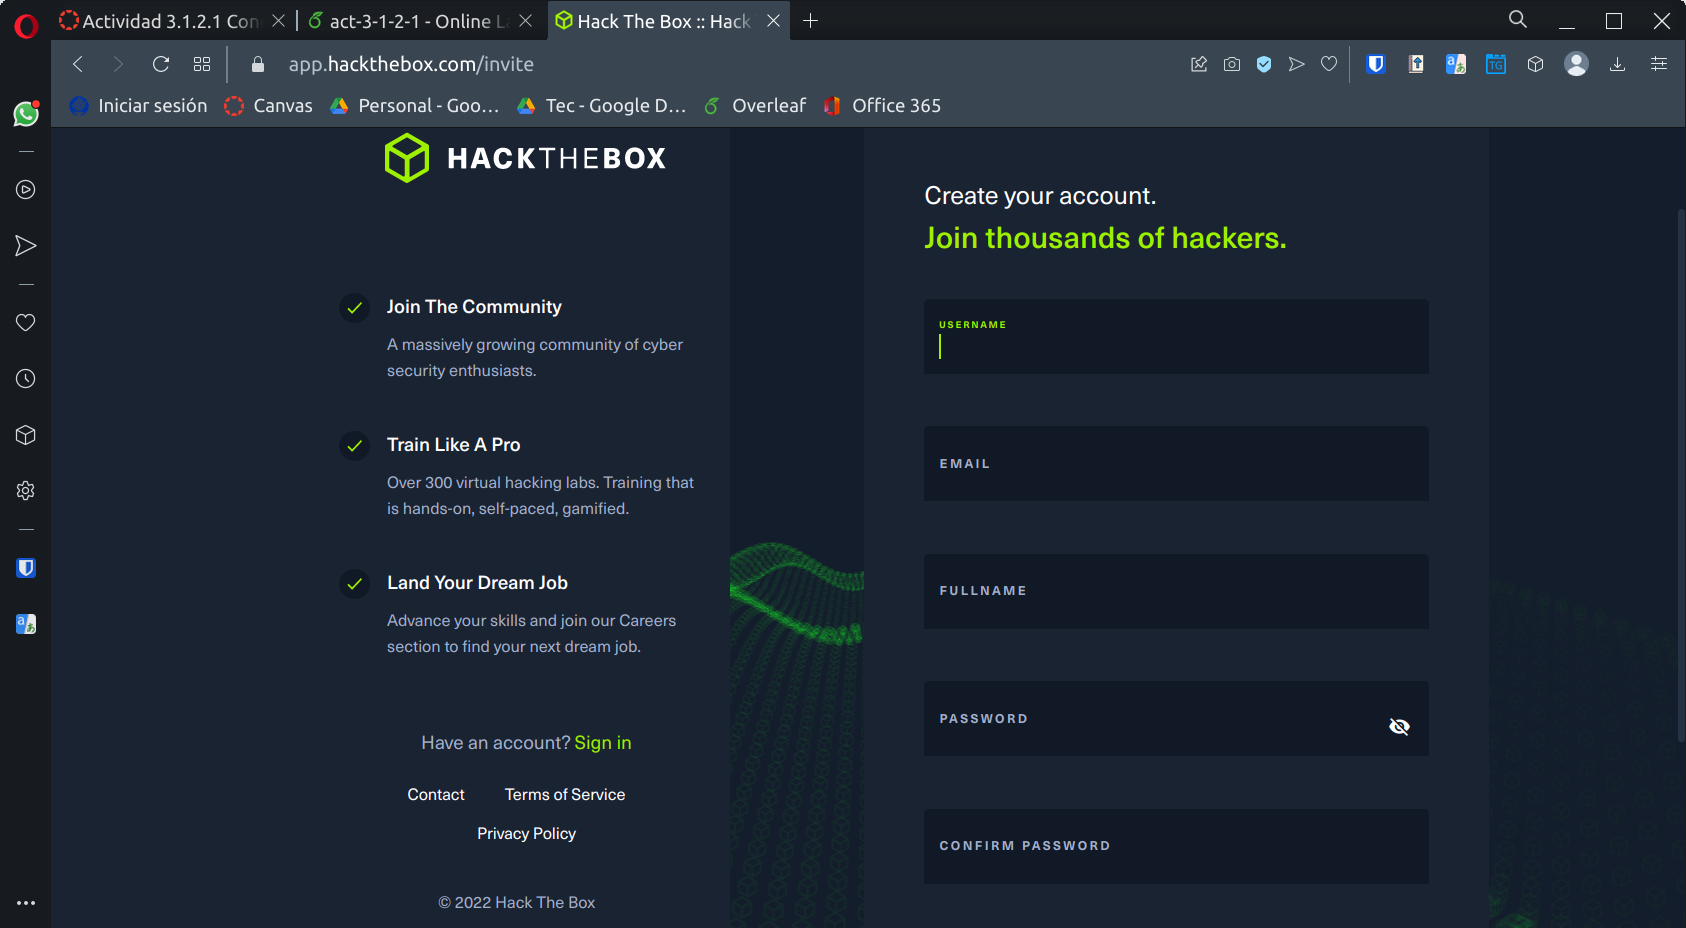
\includegraphics[scale=0.25]{img/htb-register.png}
            \caption{Ventana de registro para crear nueva cuenta en Hack the Box}
            \label{fig:registro}
        \end{figure}

        \begin{figure}[!htbp]
            \centering
            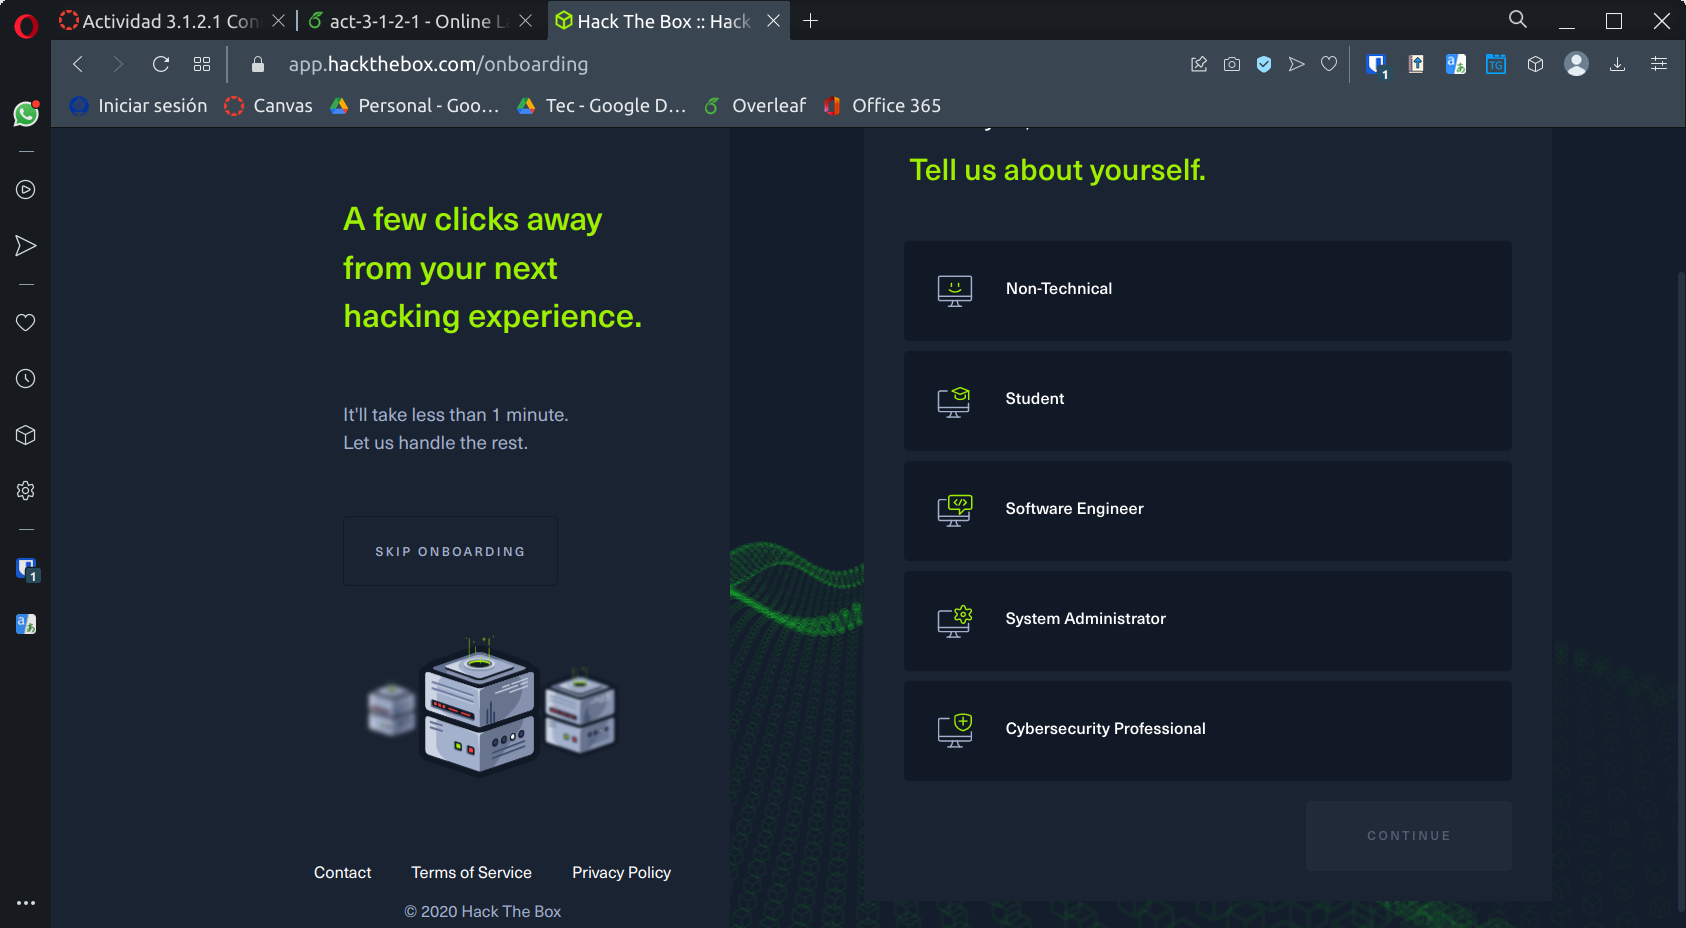
\includegraphics[scale=0.25]{img/htb-register-process.png}
            \caption{Proceso de registro en Hack the Box}
            \label{fig:proceso}
        \end{figure}

        \begin{figure}[!htbp]
            \centering
            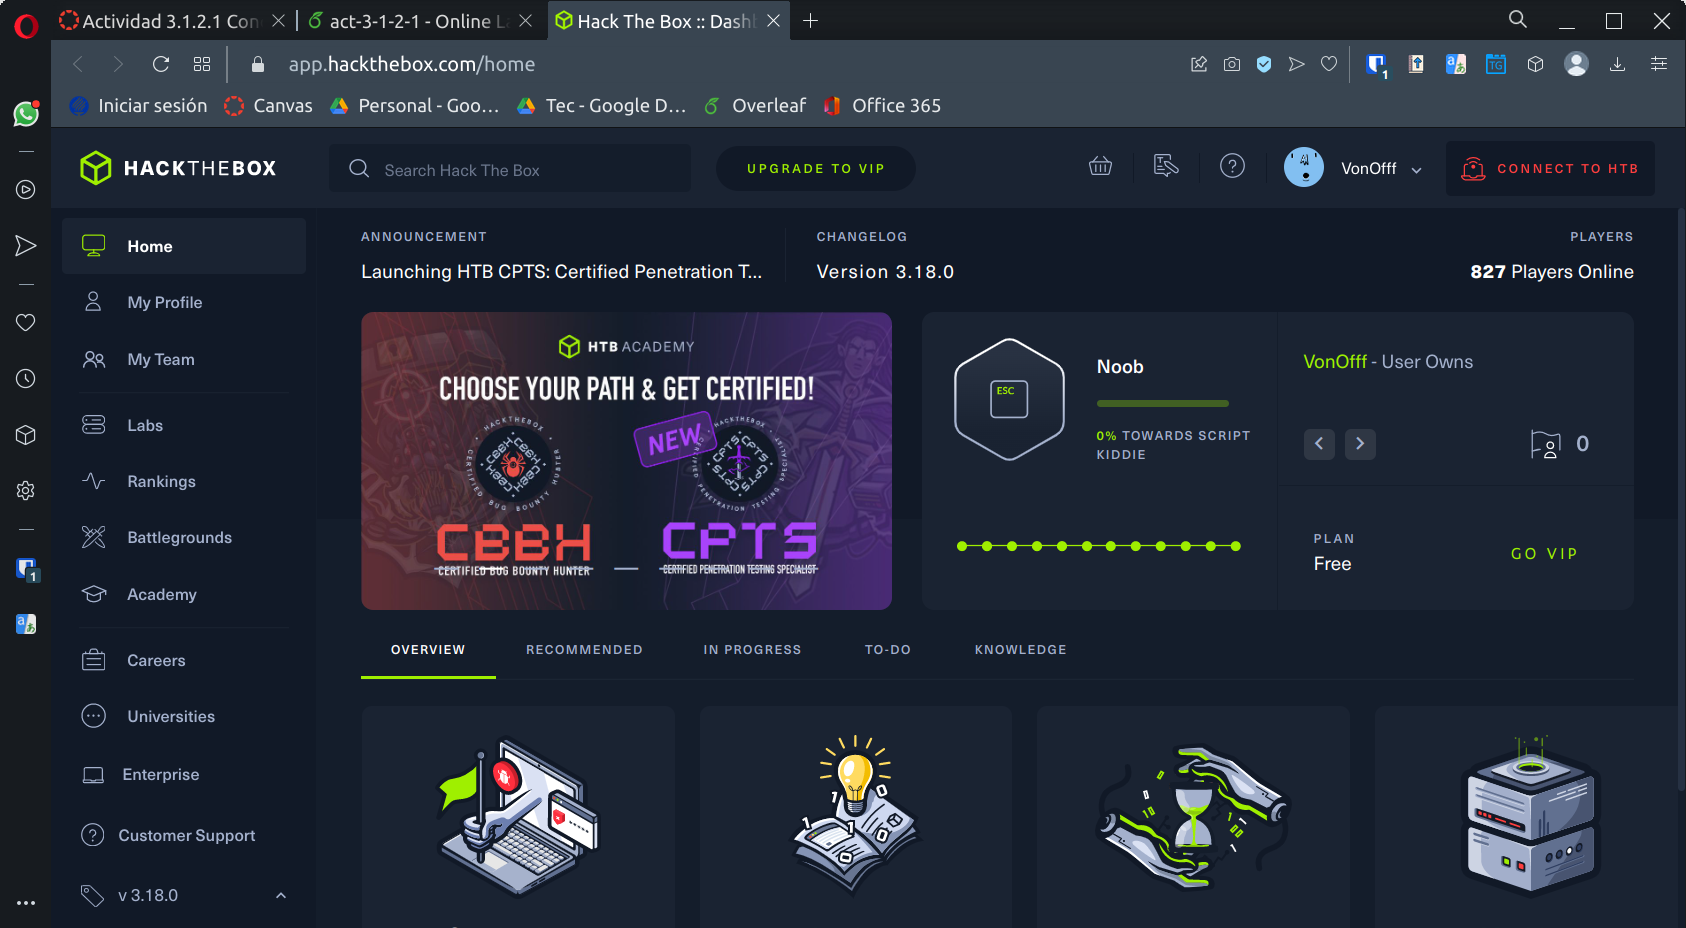
\includegraphics[scale=0.25]{img/htb-interphase.png}
            \caption{Ventana principal de Hack de Box}
            \label{fig:interfaz}
        \end{figure}

        \begin{figure}[!htbp]
            \centering
            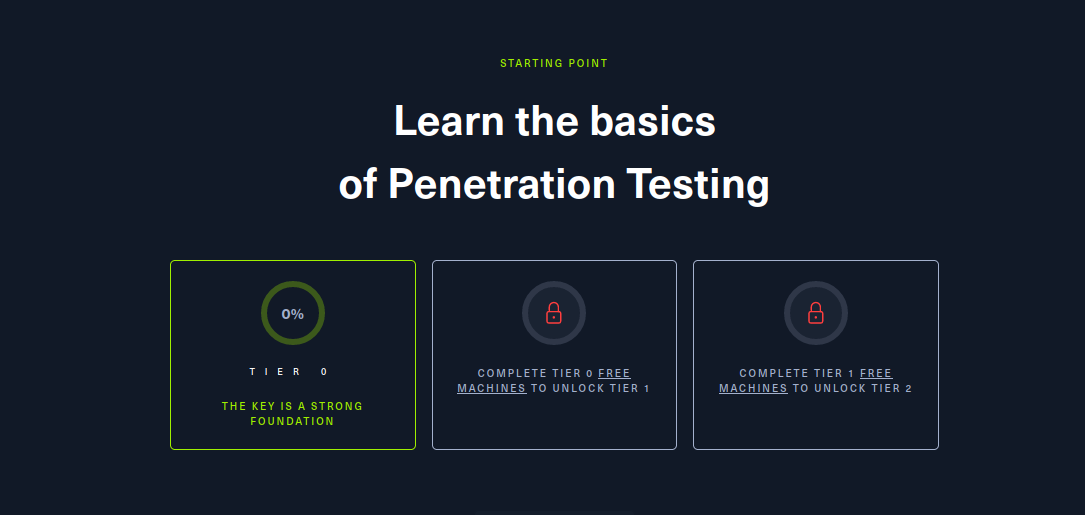
\includegraphics[scale=0.35]{img/htb-practice-welcome-screen.png}
            \caption{Primera práctica de pentest}
            \label{fig:htb-practice-welcome-screen}
        \end{figure}

        \begin{figure}[!htbp]
            \centering
            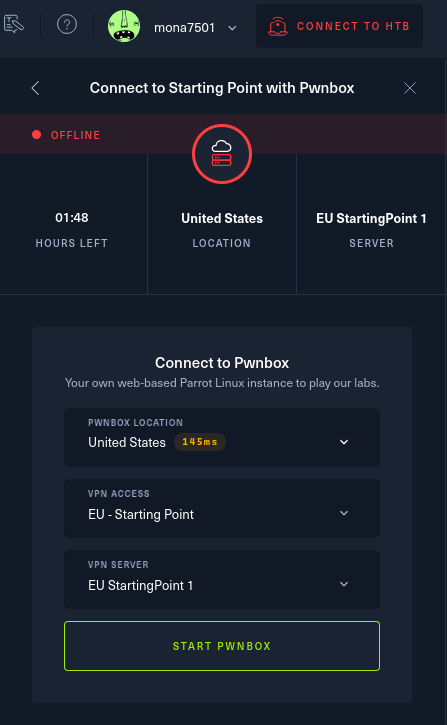
\includegraphics[scale=0.35]{img/htb-virtual-machine-setup.png}
            \caption{Configuración de máquina virtual}
            \label{fig:htb-vm-creation}
        \end{figure}

        \begin{figure}[!htbp]
            \centering
            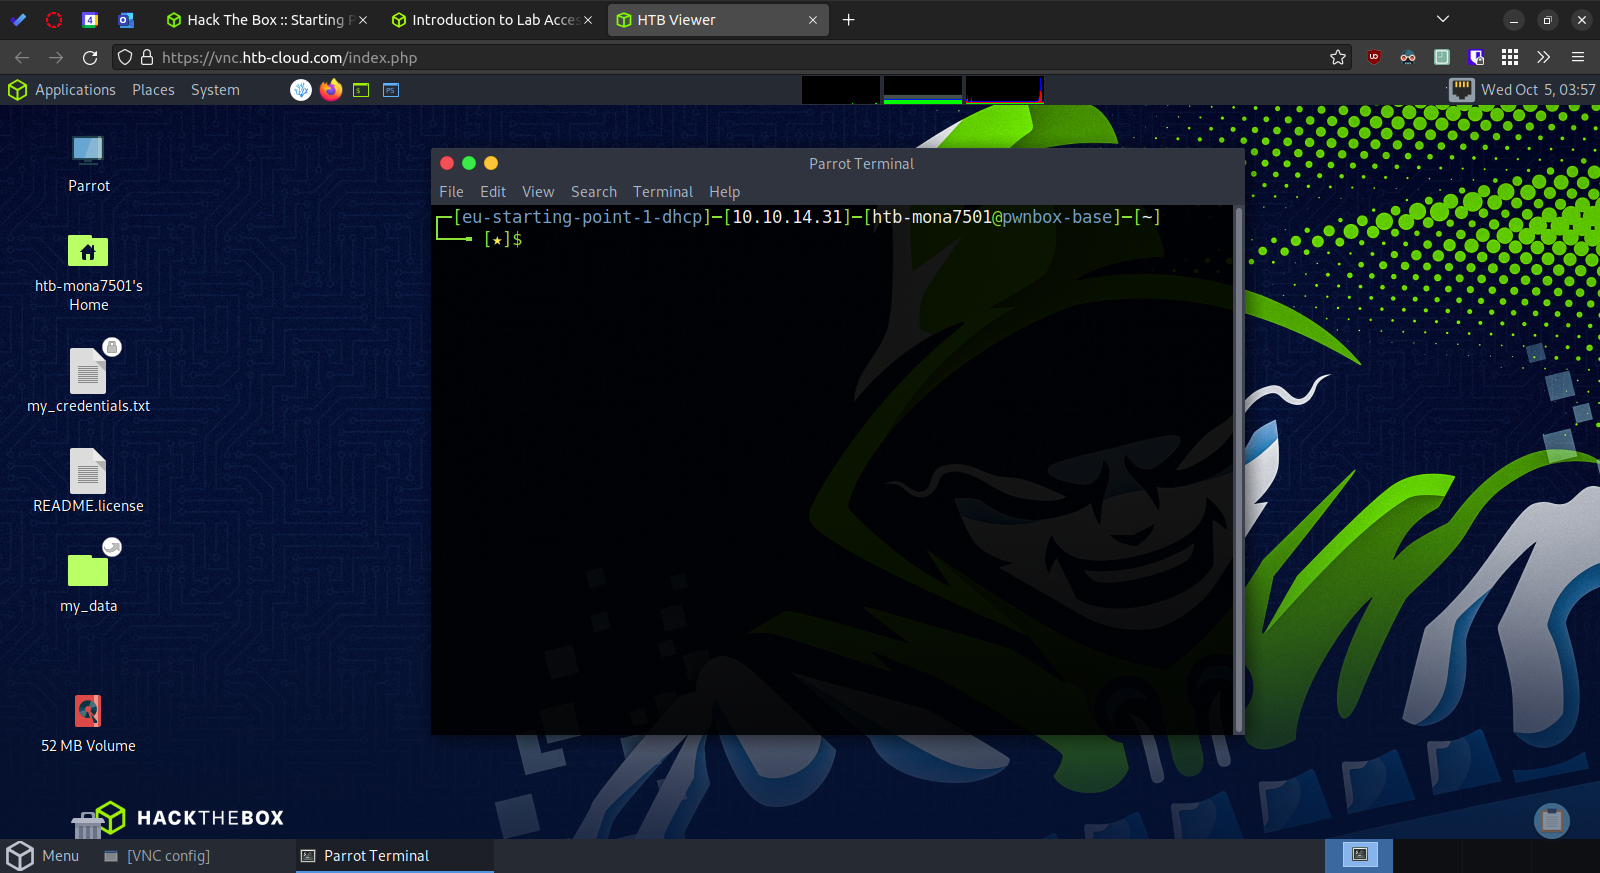
\includegraphics[scale=0.25]{img/htb-example-machine.png}
            \caption{Ejemplo de instancia de máquina virtual}
            \label{fig:htb-vm-example}
        \end{figure}

        \begin{figure}[!htbp]
            \centering
            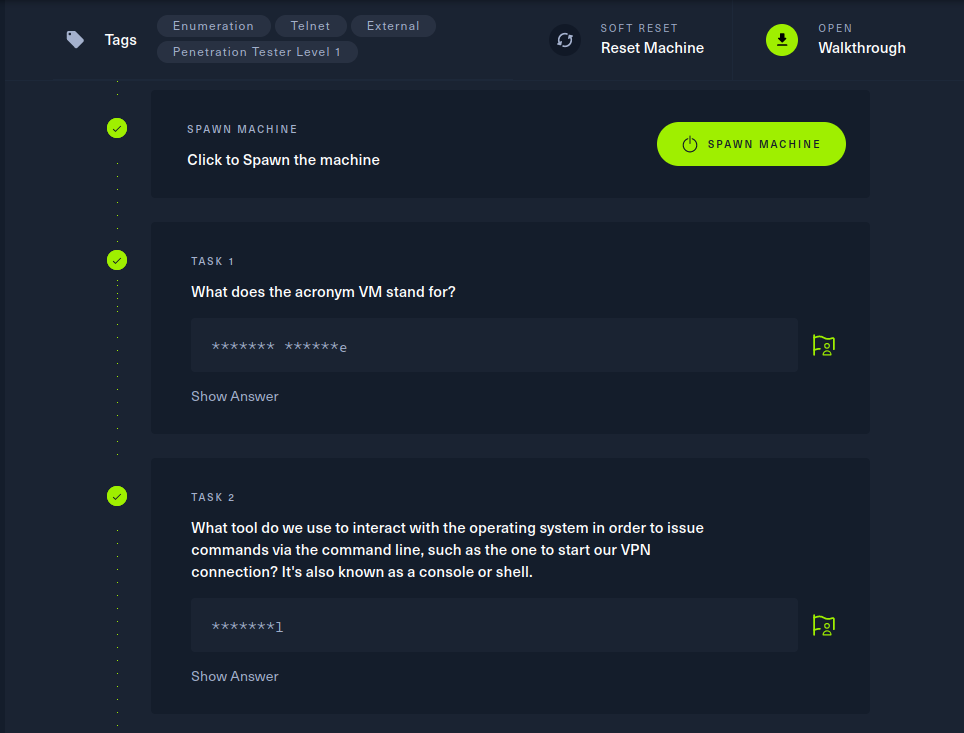
\includegraphics[scale=0.35]{img/htb-example-questionnaire.png}
            \caption{Ejemplo de preguntas de las actividades disponibles}
            \label{fig:htb-questionnaire}
        \end{figure}
        
        \begin{figure}[!htbp]
            \centering
            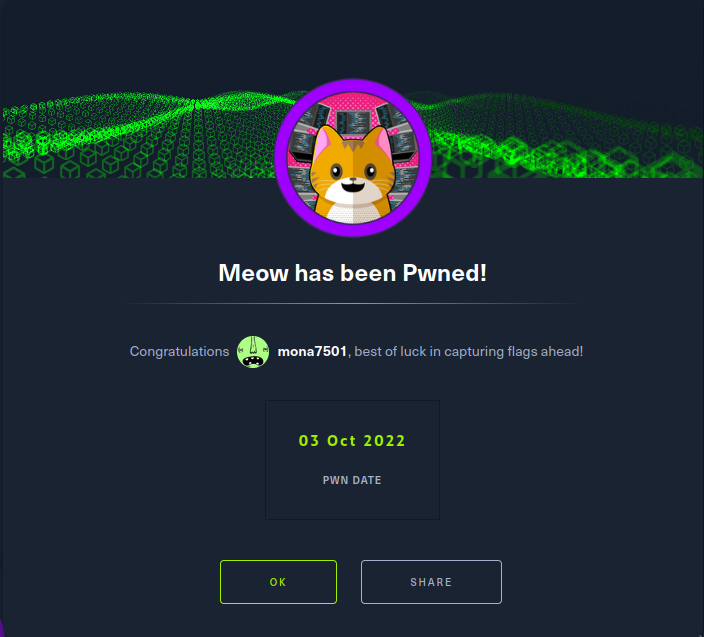
\includegraphics[scale=0.4]{img/htb-example-completion.png}
            \caption{Ejemplo de ventana de éxito en laboratorio}
            \label{fig:htb-completion}
        \end{figure}

    \clearpage
    \bibliographystyle{IEEEtran}
    \bibliography{references.bib}

\end{document}